% Green-Zone Null --- Paper C of the InceptLabs self-improvement family.
% Build: tectonic greenzone.tex   (runs bibtex passes automatically; figures are self-contained pgfplots)
% Every measured number carries a "% src:" comment to its run artifact. Small-n is stated in prose.
\documentclass[11pt]{article}
\usepackage[margin=1in]{geometry}
\usepackage{amsmath,amssymb,booktabs,graphicx,xcolor,hyperref,natbib}
\usepackage{tikz,pgfplots}\pgfplotsset{compat=1.18}
\usepackage{colortbl,array}
\usepackage{enumitem}
\hypersetup{colorlinks=true,linkcolor=blue,citecolor=blue,urlcolor=blue}
\definecolor{gz}{RGB}{34,139,34}      % green
\definecolor{gzr}{RGB}{198,40,40}     % red
\definecolor{gzb}{RGB}{25,118,210}    % blue
\definecolor{gzy}{RGB}{176,125,0}     % amber
\definecolor{cok}{RGB}{223,240,216}   % table green
\definecolor{cno}{RGB}{250,230,230}   % table red
\newcommand{\Dsym}{D_{\mathrm{sym}}}
\newcommand{\Rdet}{R_{\mathrm{det}}}
\newcommand{\Ttrace}{T_{\mathrm{trace}}}
\newcommand{\Ath}{A_{\theta}}
\newcommand{\af}{\alpha_f}
\newcommand{\OK}{\cellcolor{cok}\ding{51}}
\usepackage{pifont}
\title{\textbf{Everything Green, Still Null:\\
An Algorithmic-Core Headroom Coordinate for Self-Improving Agents}\\[3pt]
\large A Clean-Oracle Scientific Domain Where the Diagnostic Apparatus\\
Predicts Compounding but Measures None}
\author{Wenhui Chen \and [RNA team]\\ InceptLabs-Shanghai}
\date{2026 --- PRELIMINARY DRAFT}
\begin{document}\maketitle

\begin{abstract}
The most complete diagnostic account of \emph{where} self-improving agents can learn now spans four
coordinates and an oracle term: domain determinism $(\Dsym,\Rdet,\Ttrace)$ separating learnable from
pseudo-learning regimes \citep{determinismmanifold}, actuation fidelity $A$ measuring whether a correct
correction controls the next execution \citep{actuation}, and an amortizable fraction $\af$ that caps
reward determinism for physical oracles while leaving closed, exact, self-checkable oracles at
$\af\!\approx\!1$ \citep{oracleresidue}. On \emph{every} one of these axes, RNA secondary-structure
inverse design under the ViennaRNA folding oracle is in the \emph{green zone}: it is learnable
($\Dsym\!=\!\Rdet\!=\!\Ttrace\!\approx\!1$), its loop is closed ($A\!\approx\!0.85$, measured on the
live LLM agent by \citealp{actuation}), and its oracle is the $\af\!\approx\!1$ clean pole where
``search amortizes cleanly.'' All three companions therefore predict that self-improvement here should
compound. We measure \textbf{null}: a three-arm memory/skill meta-learning ablation leaves the solve
set unchanged (76/75/76 of 100), with distilled skills invoked in 3/35 episodes and decisive in none.
We argue this exposes a \textbf{fifth necessary condition the apparatus omits}: the agent's transferable
algorithmic core $\Ath$ must have \emph{headroom} the loop can compound. In the green zone that headroom
is $\approx\!0$ for two composable, separable reasons: \textbf{(H1)} the harness pre-encodes the solving
procedure, so distilled memory is redundant --- a measurement artifact, removable by a reversible
de-scaffolding ablation under which the autonomous floor is statistically indistinguishable from the
scaffolded ceiling (floor $\{8,3,5\}$ vs.\ ceiling $\{6,4,3\}$ of 35 across three rounds); and
\textbf{(H2)} an $\Ath$ ceiling --- given the ideal environment (rich diagnosis, an operator library, an
exact verifier) the agent \emph{exercises} $\Ath$ (0/52 invalid decisions) but does not \emph{exceed} a
trivial hand-coded policy (2/6 vs.\ 3/6, complementary). Using the discovery-vs-search criterion of
\citet{wangbuehler2026}, the realized self-improvement is \emph{search} (residual beyond functorial
transport $=0$): $56$ of $65$ solves are the LLM orchestrating a classical solver. This fills the
family's own named missing testbed --- a naturally-occurring, end-to-end LLM self-improvement loop on a
learnable, clean-oracle domain, null for a reason that is neither low determinism, nor an unclosed loop,
nor oracle residue. We state the result as existence-plus-mechanism and are explicit about the power
this preliminary evidence does and does not carry.
\end{abstract}

\section{Introduction}
A self-improving agent converts its own experience into standing competence: it reflects on failures,
rewrites playbooks, distils skills, and patches its scaffold, so that later tasks are solved more often
or more cheaply. Yet the capability curve often refuses to climb --- a pattern documented across
context/memory learning \citep{zhang2025ace}, weight-space RL \citep{yue2025rlvr,wu2025leash}, and
autonomous-scientist systems. The field has responded with a diagnostic program that asks not
\emph{whether} a given loop improves but \emph{where}, as a function of the domain and the system, it
\emph{can}. That program has converged on a small coordinate system, and the present paper takes it at
its word and then walks off its edge.

\paragraph{The boundary.} Three companion analyses supply the coordinates.
\citet{determinismmanifold} give three domain \emph{determinisms} --- data purity $\Dsym$, reward
determinism $\Rdet$, trace fidelity $\Ttrace$ --- and a threshold $\tau$ below which a domain is
\emph{unlearnable} (the \emph{pseudo-learning regime}: the loop fits evaluation noise and the curve
stays flat no matter how sophisticated the reflection). \citet{actuation} add the \emph{actuation}
coordinate $A=P(\text{a correctly diagnosed correction controls the next execution})$, factored
$A=A_{\mathrm{harness}}\times A_{\mathrm{model}}$; a collapsed $A$ is an \emph{unclosed loop} --- the
credit signal is computed and then dropped before it changes behaviour. \citet{oracleresidue} add the
\emph{amortizable fraction} $\af$, writing reward determinism as $\af+q_f(B)(1-\af)<1$: physical oracles
(DFT, experiment) are capped strictly below one, while \emph{closed, exact, self-checkable} oracles
(games, code, formal math) sit at the positive pole $\af\!\approx\!1$, ``where search amortizes cleanly
into weights.'' Read together, these axes carve a \emph{green zone}: a domain whose determinisms clear
$\tau$, whose loop is closed, and whose oracle is amortizable is a domain where self-improvement is
predicted to \emph{compound}.

\paragraph{The crack.} We study a domain that is green on \emph{all} of them and find that it does not
compound. RNA secondary-structure inverse design under the ViennaRNA folding oracle is, by each
companion's own placement, learnable ($\Dsym\!=\!\Rdet\!=\!\Ttrace\!\approx\!1$), loop-closed on the
live LLM agent ($A\!\approx\!0.85$; \citealp{actuation}), and oracle-amortizable ($\af\!\approx\!1$; the
clean pole of \citealp{oracleresidue}). We take these numbers from the owning companions and do not
re-derive them. On this domain, memory/skill self-improvement measures \textbf{null}. Crucially, this
is not a domain the companions overlooked: it is their \emph{explicitly named missing testbed}.
\citet{determinismmanifold} write that ``a naturally low-improvement LLM self-improvement loop on a
learnable family \dots{} remains the missing testbed'', and \citet{actuation} note that their RNA causal
claim runs on a \emph{classical} local-search executor, ``not a single end-to-end causal claim on an LLM
self-improving agent.'' We supply exactly that: a natural, end-to-end LLM loop, null for a reason none
of the four coordinates can see.

\paragraph{The claim.} We argue the null exposes a \textbf{fifth necessary condition the apparatus
omits}: the agent's transferable algorithmic core $\Ath$ --- its reasoning, search, and planning, in the
Cognitive-Core decomposition $a_t\sim\pi_\theta(a_t\mid q,C_t,K_\theta,\Ath,V)$ --- must have
\emph{headroom} that the loop can compound. Headroom is a property of the \emph{core}, orthogonal to the
domain determinisms ($\Dsym,\Rdet,\Ttrace$), to the delivery path ($A$), to the oracle ($\af$), and to
where improvement is stored (the weights/context/harness substrate axis of
\citealp{determinismmanifold}). In the green zone this headroom is $\approx\!0$, and it is zero for two
composable, \emph{separable} reasons that a reversible de-scaffolding instrument tells apart:
\textbf{H1}, the harness has pre-encoded the solving procedure, so distilled memory is redundant (a
measurement artifact); and \textbf{H2}, the agent's exercised $\Ath$ already sits at a ceiling
at-or-below a trivial hand-coded policy (a capability fact). We make headroom-consumption
\emph{measurable} by adopting (and only adopting) the retrieval/search/discovery criterion of
\citet{wangbuehler2026}: the realized self-improvement is \emph{search}, its residual beyond functorial
transport is zero, and so there was nothing to compound.

\paragraph{Contributions.}
\begin{enumerate}[leftmargin=1.4em,itemsep=1pt,topsep=2pt]
\item A \textbf{fifth necessary condition} --- \emph{algorithmic-core headroom} --- that the
  $(\Dsym,\Rdet,\Ttrace,A,\af)$ apparatus omits, exhibited by a \textbf{green-zone null}
  (\S\ref{sec:green}--\S\ref{sec:null}).
\item A \textbf{decomposition} of the zero-headroom into \textbf{H1} (scaffold-encoded procedure, a
  measurement artifact) and \textbf{H2} (an $\Ath$ ceiling, a capability fact), separated by a reversible
  de-scaffolding ablation (\S\ref{sec:mech}).
\item An \textbf{operationalization} of headroom-consumption via discovery-vs-search
  \citep{wangbuehler2026}: the realized improvement is search, residual $=0$ (\S\ref{sec:mech}).
\item A result that \textbf{fills the family's own named missing testbed} --- a natural, end-to-end LLM
  loop on a learnable, clean-oracle domain, null for a reason that is neither low determinism, nor an
  unclosed loop, nor oracle residue (throughout).
\end{enumerate}
We are explicit that this is an \emph{existence + mechanism} result at small $n$ (\S\ref{sec:limits}),
not a certified rate; the strongest-powered claim (the de-scaffolding indistinguishability, $n\!=\!3$
rounds) we lead with, and the rest we scope as existence.

\section{Setup: RNA Inverse Design under an Exact Oracle}\label{sec:setup}
\paragraph{Task.} Given a target secondary structure in dot-bracket notation, design an RNA sequence
over $\{A,C,G,U\}$ whose minimum-free-energy (MFE) fold under ViennaRNA 2.7.2
\citep{lorenz2011viennarna} (Turner2004, $37^\circ$C, dangles$=$2) string-equals the target. ``Solved''
means design-correct under the folding oracle only; it implies nothing in vivo. We evaluate on
Eterna100-V2 \citep{andersonlee2016eterna,eterna100v2}, the 100 community puzzles redesigned for the
Vienna-2 engine, spanning $12$--$400$\,nt with lone pairs, large internal loops, and intricate
multiloops.

\paragraph{Why this is a positive control.} The oracle is the reason we chose the domain: it is
\emph{free} (milliseconds), \emph{exact} (the fold is the reward), and \emph{self-checkable} (the agent
can verify its own candidate without paying an external oracle). In the language of
\citet{oracleresidue} this is the $\af\!\approx\!1$ clean-oracle pole --- the opposite of a physical
DFT oracle --- so there is no amortization residue on the reward channel and the residual difficulty
(search) is of the \emph{amortizable} kind. Any null here therefore indicts the \emph{mechanism}, not
the domain.

\paragraph{The agent and its harness.} The subject is an openclaude agent \citep{openclaude} driven by
GLM-5.2, exposed to a bounded RNA toolset (fold/verify/diagnose primitives, a many-restart
\texttt{inverse\_fold} search, a decomposition helper) plus the general agentic toolset (Bash, code
execution, memory, sub-agents). Its memory is either a declarative \emph{memory directory} ($K_\theta$
content) or a growing library of invocable \emph{Skills} ($\Ath$ procedure). Distillation of experience
into either vehicle is guarded by a red line, structurally enforced: distilled artifacts are masked of
all sequences and structures before writing, so memory can carry \emph{procedure}, never answers, and
web search is disabled so no external solution can leak.

\section{The Green Zone}\label{sec:green}
We place RNA-under-ViennaRNA on each companion axis, taking every value from the owning companion
(Table~\ref{tab:coords}, Figure~\ref{fig:coords}). The determinisms are maximal: the reward is the exact
fold ($\Rdet\!\approx\!1$), the learned-from object is the structure itself and re-instantiates
identically ($\Dsym\!\approx\!1$), and every attempt is fully attributable to its fold
($\Ttrace\!\approx\!1$), so $\min(\Dsym,\Rdet,\Ttrace)\gg\tau$ and \citet{determinismmanifold} place the
domain firmly in the learnable region. The loop is closed: \citet{actuation} measure a natural actuation
fidelity of $A\!\approx\!0.85$ on the live LLM agent (DeepSeek-V4-pro $0.86$, GLM-5.2 $0.86$, Sonnet-5
$0.85$), well above the unclosed-loop regime. And the oracle is amortizable: RNA-under-ViennaRNA
\emph{is} the closed/exact/self-checkable pole at which \citet{oracleresidue} state ``search amortizes
cleanly into weights,'' $\af\!\approx\!1$. By every axis the domain is green; every companion predicts
compounding.

\begin{table}[t]\centering\small
\caption{RNA-under-ViennaRNA on the family's coordinate system. Every value is taken from the owning
companion (cited, not re-derived). All axes clear; the fifth (headroom) is this paper's subject.}
\label{tab:coords}
\begin{tabular}{@{}llll@{}}
\toprule
Coordinate & Meaning & RNA value & Owner / verdict\\
\midrule
$\Dsym$ & data purity & $\approx 1$ & \citep{determinismmanifold} \;learnable\\
$\Rdet$ & reward determinism & $\approx 1$ (exact fold) & \citep{determinismmanifold} \;learnable\\
$\Ttrace$ & trace fidelity & $\approx 1$ & \citep{determinismmanifold} \;learnable\\
$A$ & actuation fidelity & $\approx 0.85$ (live LLM) & \citep{actuation} \;loop closed\\
$\af$ & oracle amortizability & $\approx 1$ (clean pole) & \citep{oracleresidue} \;amortizable\\[2pt]
\rowcolor{cno}\textbf{headroom} & \textbf{$\Ath$ compoundable} & \textbf{$\approx 0$ (this work)} & \textbf{binds; \S\ref{sec:coord}}\\
\bottomrule
\end{tabular}
\end{table}

\begin{figure}[t]\centering
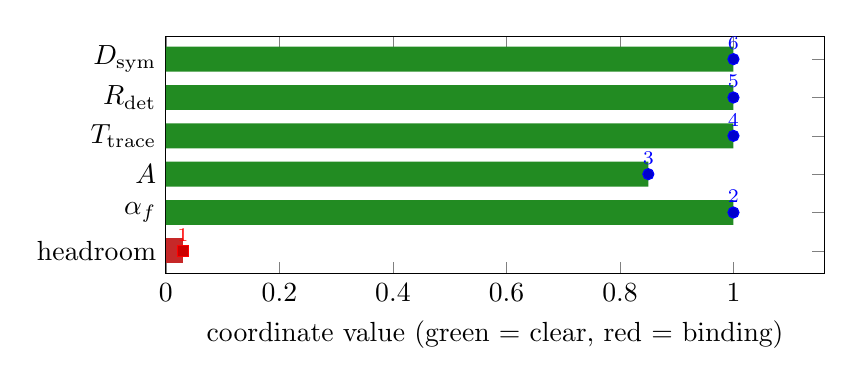
\begin{tikzpicture}
\begin{axis}[width=.82\linewidth,height=4.6cm,xmin=0,xmax=1.16,ymin=0.4,ymax=6.6,bar width=9pt,
  ytick={1,2,3,4,5,6},yticklabels={headroom,$\af$,$A$,$\Ttrace$,$\Rdet$,$\Dsym$},
  xlabel={coordinate value (green = clear, red = binding)},
  nodes near coords,nodes near coords style={font=\scriptsize},every axis plot/.append style={draw=none}]
\addplot+[xbar,bar shift=0pt,fill=gz] coordinates {(1,6)(1,5)(1,4)(0.85,3)(1,2)};
\addplot+[xbar,bar shift=0pt,fill=gzr] coordinates {(0.03,1)};
\end{axis}
\end{tikzpicture}
\caption{The argument in one view. Every companion coordinate for RNA-under-ViennaRNA is clear (green);
the fifth axis this paper names --- algorithmic-core headroom --- is at the floor (red). Values cited
from \citet{determinismmanifold,actuation,oracleresidue}.}
\label{fig:coords}
\end{figure}

\section{The Fifth Coordinate: Algorithmic-Core Headroom}\label{sec:coord}
An action conditions on the Cognitive-Core tuple
$a_t\sim\pi_\theta(a_t\mid q,C_t,K_\theta,\Ath,V)$: parametric knowledge $K_\theta$, an algorithmic core
$\Ath$ (transferable reasoning/search/planning), working memory $C_t$, and a verifier $V$. The four
family coordinates each attach to a different one of these. The determinisms are properties of the
\emph{domain} (they govern what $V$ and the trace can certify); $A$ is a property of the \emph{delivery
path} from a computed correction to $C_t$ and behaviour; $\af$ is a property of the \emph{oracle} $V$;
and the substrate taxonomy of \citet{determinismmanifold} is a property of \emph{where} an improvement
is stored ($B_W$/$B_C$/$B_H$). None of these is a property of $\Ath$ itself. We propose the missing
condition:
\begin{quote}
\emph{Algorithmic-core headroom.} A self-improvement loop compounds only if the agent's algorithmic core
$\Ath$ has capability that the accumulation can add \emph{beyond what is already available to the
policy}. A domain green on $(\Dsym,\Rdet,\Ttrace,A,\af)$ may still have headroom $\approx0$, and then the
loop compounds nothing, however clean the domain, loop, and oracle.
\end{quote}
Headroom is orthogonal to all four axes and to the substrate axis; it can be low while every other axis
is high, which is precisely the regime we exhibit.

\paragraph{Measuring headroom consumption (borrowed instrument).} We adopt --- and only adopt ---
the categorical criterion of \citet{wangbuehler2026}, which separates \emph{retrieval} (an artifact
already in the schema), \emph{search} (a new artifact within a fixed schema, a provenance-preserving
update), and \emph{discovery} (a verified regime transition whose content is the \emph{residual beyond
the left-Kan functorial transport} of prior artifacts). A self-improvement loop consumes headroom only
if its accumulation produces \emph{discovery}; if the accumulation is functorial \emph{transport}
(residual $=0$), the headroom it had to compound was already zero. We claim none of this machinery as
ours; we use the residual-beyond-transport test as an instrument to read our data.

\section{The Green-Zone Null}\label{sec:null}
\paragraph{Protocol.} We run one agent with one seeded memory directory across three arms that differ
\emph{only} in what is written between epochs, holding the agent, seed, tools, task set, and budget
fixed: \textsc{frozen} (nothing is written; control), \textsc{accumulate} ($K_\theta$ content bullets
distilled into the memory directory), and \textsc{askill} ($\Ath$ distilled into invocable openclaude
Skills). Epoch~1 is identical across arms (the \textsc{askill} skill library starts empty); the arms
then iterate for four epochs on the $35$ Eterna100-V2 puzzles unsolved at a $65$-solve baseline. The
between-epoch write is the only free variable, so the gap $\Delta=\textsc{askill}-\textsc{frozen}$ after
epoch~4 is exactly the procedural-memory meta-learning effect.

\paragraph{Result: null.} The final solved sets are \textbf{76 / 75 / 76} of 100 for
\textsc{frozen}/\textsc{accumulate}/\textsc{askill}
(Table~\ref{tab:null}, Figure~\ref{fig:null}).% src: runs/meta_ladder_{frozen,accumulate,askill}/epoch_progress.json
The three arms land within one of one another; $\Delta=0$. A mechanism check is decisive about
\emph{why}: the \textsc{askill} arm invoked the \texttt{Skill} tool in only \textbf{3/35} episodes, all
on tasks it did not solve, and \emph{none} of its eleven solves used a distilled skill. In a domain
green on every companion axis, strategy recall is not a binding lever: the accumulation had no headroom
to compound.

\begin{table}[t]\centering\small
\caption{The green-zone null. Three arms, identical agent/seed/tools/tasks; only the between-epoch
write differs. Final solved of 100 (from a 65 baseline).}
\label{tab:null}
\begin{tabular}{@{}llcc@{}}
\toprule
Arm & externalizes & solved / 100 & skills invoked\\
\midrule
\textsc{frozen} (control) & --- & \textbf{76} & ---\\
\textsc{accumulate} & $K_\theta$ content & \textbf{75} & ---\\
\textsc{askill} & $\Ath$ skills & \textbf{76} & \textbf{3/35, 0 decisive}\\
\bottomrule
\end{tabular}
\end{table}

\begin{figure}[t]\centering
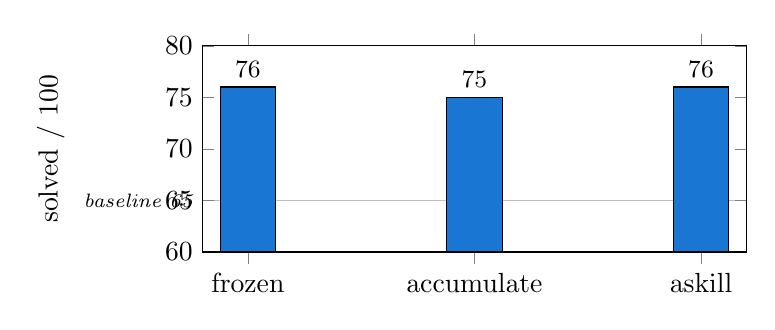
\begin{tikzpicture}
\begin{axis}[ybar,width=.7\linewidth,height=4.2cm,ymin=60,ymax=80,bar width=20pt,
  ylabel={solved / 100},symbolic x coords={frozen,accumulate,askill},xtick=data,
  nodes near coords,nodes near coords style={font=\small},
  extra y ticks={65},extra y tick labels={baseline 65},extra y tick style={grid=major,tick label style={font=\scriptsize\itshape}}]
\addplot[fill=gzb] coordinates {(frozen,76)(accumulate,75)(askill,76)};
\end{axis}
\end{tikzpicture}
\caption{Three-arm meta-learning is null: \textsc{frozen}/\textsc{accumulate}/\textsc{askill} land at
$76/75/76$, within one of each other, from a shared baseline of $65$. Distilled $\Ath$ skills were
invoked in $3/35$ episodes and decisive in none.}
\label{fig:null}
\end{figure}

\section{Why the Headroom Is Zero}\label{sec:mech}
The null of \S\ref{sec:null} is over-determined between two mechanisms. We separate them with a
reversible instrument and find both present.

\subsection{H1: Scaffold-Encoded Procedure (a Measurement Artifact)}\label{sec:h1}
An audit of the harness finds the full solving procedure inlined in the tool layer: a
\textsc{decompose}$\to$\textsc{design}$\to$\textsc{stitch}$\to$\textsc{repair} recipe appears in the
agent prompt, in the MCP tool docstrings, and in the distilled skills alike. The distilled skills merely
restate what the scaffold already provides, so there is nothing new to retrieve --- the null is, in
part, a \emph{redundancy artifact}: the loop measures null because the procedure it would learn is
already delivered.

We test this with a single reversible flag, \texttt{RNA\_AUTONOMOUS}, that strips the procedure from the
tool layer down to neutral primitives (fold, verify, diagnose, generic restart-search), replaces the
solver-calling scaffolds with facts-only tool renderings, and empties the seeded memory --- while
leaving the flag-off harness byte-identical (a mirror unit test guards this). If the scaffold carried
genuine capability, the de-scaffolded \emph{floor} should fall far below the scaffolded \emph{ceiling}.
Across three rounds on the same $35$ hard-tail targets, at matched per-episode budget and identical
denominator (raw solve-rate, no baseline add), the ceiling (scaffolded) solves $\{6,4,3\}$ (mean
$4.33$) and the floor (autonomous) solves $\{8,3,5\}$ (mean
$5.33$)% src: runs/p1_logs/p1_{ceiling,floor}_tail35_r{1,2,3}.log
--- \emph{statistically indistinguishable}, with the floor if anything higher, and single-round variance
($3$--$8$ of $35$) swamping the between-arm difference (Figure~\ref{fig:mech}, left; per-round detail in
Appendix~\ref{app:descaffold}). Head-to-head, the scaffold buys no measurable capability on the hard
tail.

\paragraph{A retracted single-point estimate.} An earlier reading of one round --- floor $3/35$ against
a scaffolded $11/35$ --- suggested that $\sim\!73\%$ of hard-tail capability was scaffolding. That figure
does not survive the three-round replication and we \emph{retract} it. The honest statement is
weaker and more useful: on the hard tail the scaffold's contribution is within round-to-round noise, and
single-point self-improvement estimates mislead --- itself a cautionary datum for the field's habit of
reporting one number per configuration.

\subsection{H2: An $\Ath$ Ceiling (a Capability Fact)}\label{sec:h2}
Redundancy (H1) explains why memory adds nothing \emph{on top of} the scaffold, but not whether the
agent's own core could improve if handed the ideal environment. To test H2 we build that environment: a
\emph{self-revising} solver loop in which, each step, the exact oracle emits a rich diagnosis (per-pair
formation probability from the partition function, contiguous defect regions, ensemble defect) and the
LLM \emph{itself} selects the next operator from a fixed library --- many-restart inverse-fold, a
hierarchical decompose-and-assemble, a weak-stem GC-strengthener, and a targeted endgame that closes the
exact unformed pairs --- with the verifier scoring every step. This is the agent playing the role of a
hand-coded selection policy, and nothing else; it isolates the operator-\emph{selection} facet of $\Ath$.

We compare the LLM-driven controller against a trivial hand-coded diagnosis$\to$operator policy
(\textsc{greedy}: at small bp-distance pick the endgame operator, at low pair-probability pick the
strengthener, at many defect regions re-decompose, else restart) on the six discriminating short-hard
targets, two seeds each (Table~\ref{tab:agent}, Figure~\ref{fig:mech}, right). The agent \emph{exercises}
$\Ath$: \textbf{0/52} of its decisions were invalid, and its stated reasons are coherent (``$bp\!=\!1$
near-miss, close the exact unformed pair''; operator-choice profile in Appendix~\ref{app:ops}). But it
does not \emph{exceed} the trivial policy: \textsc{greedy} cracks \textbf{3/6}, the agent
\textbf{2/6},% src: runs/self_revise_agent/agent_compare.json
and --- decisively for the ``competitive but not superior'' reading --- the two are \emph{complementary,
not nested}: the agent uniquely cracks one target \textsc{greedy} fails, \textsc{greedy} uniquely cracks
two the agent fails, and two are beyond both. Given the ideal environment, the agent's selection-$\Ath$
reaches a competitive-but-not-superior operating point relative to a hand-coded policy. There is no
residual capability above a trivial baseline for memory to compound.

\begin{table}[t]\centering\small
\caption{H2, the $\Ath$ ceiling. Six discriminating short-hard targets; agent-driven operator selection
vs.\ a trivial hand-coded \textsc{greedy} policy, same operator library and budget, two seeds each.
Not nested --- the agent uniquely cracks 62; \textsc{greedy} uniquely cracks 66, 57.}
\label{tab:agent}
\setlength{\tabcolsep}{5pt}
\begin{tabular}{@{}rllcc@{}}
\toprule
pid & len & puzzle & \textsc{greedy} & agent\\
\midrule
49 & 101 & Kudzu                 & \OK & \OK\\
66 &  36 & Bug 38                & \OK & \cellcolor{cno}\ding{55}\\
57 &  44 & multilooping fun      & \OK & \cellcolor{cno}\ding{55}\\
62 &  53 & Bug 18                & \cellcolor{cno}\ding{55} & \OK\\
65 &  40 & Branching Loop        & \cellcolor{cno}\ding{55} & \cellcolor{cno}\ding{55}\\
61 &  69 & Chicken feet          & \cellcolor{cno}\ding{55} & \cellcolor{cno}\ding{55}\\
\midrule
\multicolumn{3}{@{}l}{\textbf{cracked / 6}} & \textbf{3} & \textbf{2}\\
\multicolumn{3}{@{}l}{invalid decisions} & --- & \textbf{0/52}\\
\bottomrule
\end{tabular}
\end{table}

\begin{figure}[t]\centering
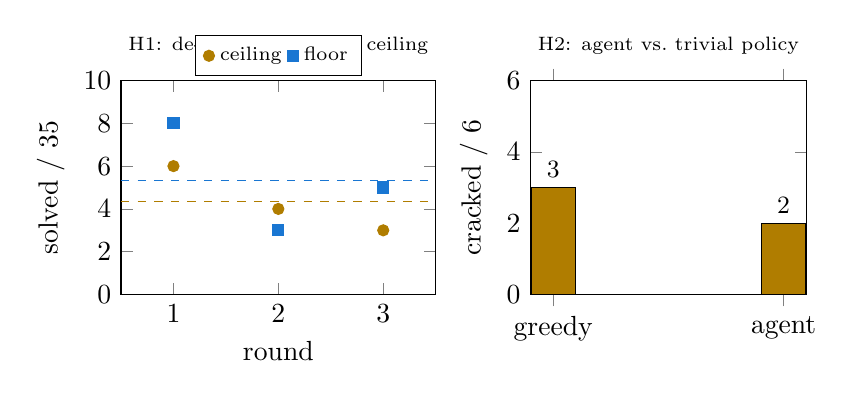
\begin{tikzpicture}
% left: de-scaffold floor vs ceiling, 3 rounds
\begin{axis}[name=ax1,width=.46\linewidth,height=4.3cm,ymin=0,ymax=10,
  ylabel={solved / 35},xtick={1,2,3},xlabel={round},xmin=0.5,xmax=3.5,
  legend style={font=\scriptsize,at={(0.5,1.02)},anchor=south,legend columns=2},title={\scriptsize H1: de-scaffold floor vs.\ ceiling}]
\addplot[only marks,mark=*,gzy] coordinates {(1,6)(2,4)(3,3)}; \addlegendentry{ceiling}
\addplot[only marks,mark=square*,gzb] coordinates {(1,8)(2,3)(3,5)}; \addlegendentry{floor}
\addplot[gzy,dashed,domain=0.5:3.5] {4.33};
\addplot[gzb,dashed,domain=0.5:3.5] {5.33};
\end{axis}
% right: agent vs greedy cracks
\begin{axis}[name=ax2,at={(ax1.east)},anchor=west,xshift=1.2cm,ybar,width=.42\linewidth,height=4.3cm,
  ymin=0,ymax=6,bar width=16pt,ylabel={cracked / 6},symbolic x coords={greedy,agent},xtick=data,
  nodes near coords,nodes near coords style={font=\small},title={\scriptsize H2: agent vs.\ trivial policy}]
\addplot[fill=gzy] coordinates {(greedy,3)(agent,2)};
\end{axis}
\end{tikzpicture}
\caption{The two mechanisms of zero headroom. \emph{Left (H1):} across three rounds the de-scaffolded
floor (blue) is indistinguishable from the scaffolded ceiling (amber); dashed lines are means
($5.33$ vs.\ $4.33$), single-round variance swamps the gap. \emph{Right (H2):} given the ideal
environment, the agent's selection-$\Ath$ ($2/6$) is competitive-but-not-superior to a trivial policy
($3/6$), and complementary (Table~\ref{tab:agent}).}
\label{fig:mech}
\end{figure}

\subsection{The Realized Improvement Is Search, Not Discovery}\label{sec:search}
We attribute the $65$-solve baseline by winning-sequence provenance. \textbf{56 of 65} solves were
carried by an automated inverse-fold / simulated-annealing solver that the LLM \emph{orchestrated} ---
$37$ via the harness search tools, $16$ via the agent's own scripted \texttt{RNA.inverse\_fold} in a
Bash cell, $3$ via a self-written annealer --- and only $9$ were hand-designed from
scratch.% src: provenance scan
In the terms of \citet{wangbuehler2026}, the agent's realized capability is a within-schema \emph{search}
orchestrated by judgment, not a schema transition: its residual beyond functorial transport is zero.
That is exactly why the memory loop had no discovery to compound --- there was no new representational
content for accumulation to carry forward, only the same search re-invoked.

\subsection{The Residual Is the Oracle's, Not the Agent's}\label{sec:residual}
Finally, the $24$ unsolved Eterna100-V2 targets are genuinely solver-hard, so the null is not masking a
reachable win the agent is fumbling. Our strongest available solver reaches bp$=0$ on a $258$-nt target
only via a $24$-minute brute-force hill-climb, and fails a $108$-nt short-hard target at bp$=6$ after
$13.5$ minutes; the public state of the art, DesiRNA \citep{wirecki2025desirna}, reaches $97/100$ only at
$\sim\!24$\,h per puzzle ($85/100$ under a minute, $95/100$ under an hour). This residual is the
$\af\!\approx\!1$ clean-oracle \emph{compute} wall of \citet{oracleresidue} --- amortizable in principle,
unpaid within budget --- which we cite as theirs, not as a contribution here. Budget-aligned, the honest
classical comparison at minute-scale is $\sim\!85$ vs.\ our $76$ (Table~\ref{tab:sota},
Figure~\ref{fig:sota}); pushing to $97$ buys the last two puzzles with $\sim\!24$\,h each and is a
compute problem, not a self-improvement one.

\begin{table}[t]\centering\small
\caption{Public Eterna100-V2 anchors (deep-research verified). ``90/99'' mistransmissions corrected:
$99$ is Montparnasse on V1; $90$ is a weakened fixed-budget NEMO baseline.}
\label{tab:sota}
\begin{tabular}{@{}llll@{}}
\toprule
method & V2 & budget & class\\
\midrule
DesiRNA \citep{wirecki2025desirna} & \textbf{97} & $\sim$24\,h/puzzle & classical REMC\\
DesiRNA (budget-matched) & $\sim$85 & $<$1\,min/puzzle & classical REMC\\
NEMO (native) & $\sim$94 & long MC & classical\\
LLM-method SOTA \citep{gautam2026rnalm} & $\sim$80 & --- & LLM\\
\textbf{this work (scaffolded)} & \textbf{76} & minute-scale & LLM-orchestrated\\
this work (base, no memory) & 56 & minute-scale & LLM\\
\bottomrule
\end{tabular}
\end{table}

\begin{figure}[t]\centering
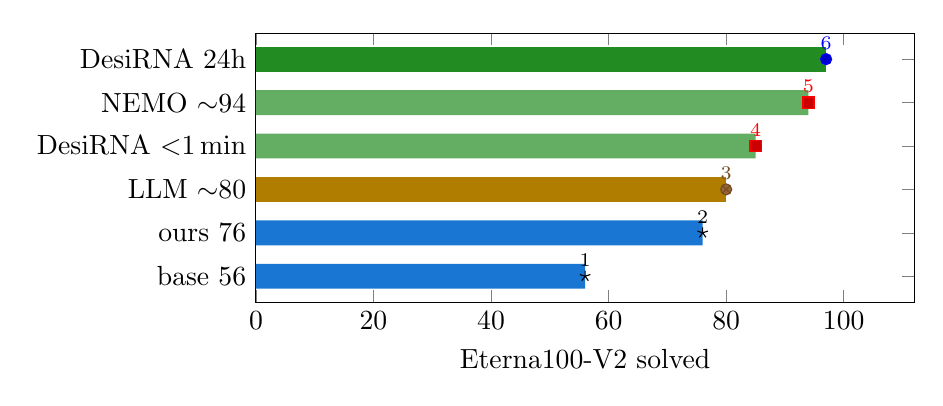
\begin{tikzpicture}
\begin{axis}[width=.82\linewidth,height=5cm,xmin=0,xmax=112,ymin=0.4,ymax=6.6,bar width=9pt,
  ytick={1,2,3,4,5,6},yticklabels={base 56,ours 76,LLM $\sim$80,DesiRNA $<$1\,min,NEMO $\sim$94,DesiRNA 24h},
  xlabel={Eterna100-V2 solved},nodes near coords,nodes near coords style={font=\scriptsize},
  every axis plot/.append style={draw=none}]
\addplot+[xbar,bar shift=0pt,fill=gz] coordinates {(97,6)};
\addplot+[xbar,bar shift=0pt,fill=gz!70] coordinates {(94,5)(85,4)};
\addplot+[xbar,bar shift=0pt,fill=gzy] coordinates {(80,3)};
\addplot+[xbar,bar shift=0pt,fill=gzb] coordinates {(76,2)(56,1)};
\end{axis}
\end{tikzpicture}
\caption{Budget-aligned SOTA. The honest classical comparison at minute-scale is DesiRNA $\sim\!85$ vs.\
our $76$; the $97$ is a $24$-h/puzzle number. The gap is a compute wall (\citealp{oracleresidue}), not a
self-improvement one.}
\label{fig:sota}
\end{figure}

\section{Related Work}\label{sec:related}
\paragraph{The companion family (division of labour).} This is the RNA member of a five-paper program;
we state ownership so nothing is double-counted. \citet{actuation} owns the actuation coordinate $A$ ---
whether a \emph{delivered} correction is adopted --- and reports RNA's $A\!\approx\!0.85$ and a
memory-severing efficiency ablation on a \emph{classical} executor. Our fifth coordinate concerns $\Ath$
\emph{generation/orchestration} headroom, not adoption --- an orthogonal axis --- and we supply the
end-to-end LLM testbed A1 explicitly reserves as missing; we cite $A\!\approx\!0.85$ verbatim and do not
restate the severing ablation. \citet{determinismmanifold} owns $(\Dsym,\Rdet,\Ttrace)$, $\tau$, the
substrate taxonomy, and the pseudo-learning regime --- a null caused by \emph{low} determinism; our null
is in a \emph{high}-determinism domain, a different null cause, and the headroom axis is orthogonal to
the determinisms and to which substrate stores the improvement. \citet{oracleresidue} owns $\af$, the
$\Rdet$ ceiling for \emph{physical} oracles, and the judgment--computation asymmetry; we sit at its
$\af\!\approx\!1$ clean-oracle positive pole and show self-improvement can still be null there --- sourced
in $\Ath$, not the oracle --- a boundary case that \emph{completes} A3: capability can fail to eat even
already-clean knowledge when the core that would digest it is at ceiling. \citet{compoundingprofile}
adjudicates compounding-vs-amplification on SAT/A$^\ast$; we locate a headroom coordinate on a different
domain and import none of its adjudication machinery.

\paragraph{Self-improvement can be null (not our claim).} That verifiable reward is necessary but not
sufficient is documented: \citet{learnablegain2026} show task metrics rising while learnable information
is unchanged, and \citet{yue2025rlvr,wu2025leash} bound RLVR to the base model's support. ``The loop can
be null'' is therefore \emph{not} our contribution. Our delta is to (i) give the null a decomposed
\emph{mechanism} (H1/H2), (ii) give it a \emph{home} in the field's most complete
where-can-self-improve coordinate system, showing that system has a blind axis, (iii) isolate it in a
\emph{clean-exact-oracle} domain that rules out oracle, determinism, and actuation, and (iv) make
headroom-consumption \emph{measurable} via discovery-vs-search.

\paragraph{Diagnostic frameworks.} We are not proposing another test-time-improvement metric suite in
the manner of \citet{tide2026} or a metacognition ingredient \citep{metacognitive2025}; we add a
\emph{coordinate} to the where-is-improvement-possible map and pin it with a null in the all-green zone.

\paragraph{Scaffold-vs-model attribution.} A 2026 cluster decomposes agent scores across models and
harnesses --- Harness-Bench \citep{harnessbench2026}, ClawsBench \citep{clawsbench2026}, agent
psychometrics \citep{psychometrics2026}, and, nearest to us, a scientific-agent scaffold-dominance study
\citep{aiscientists2026} --- and an externalization review \citep{externalization2026} taxonomizes
memory/skills/harness. We differ by the coordinate-system placement, the clean-exact-oracle isolation,
and the discovery-vs-search criterion, rather than a score-attribution method; the discovery-vs-search
criterion itself is \citet{wangbuehler2026}'s, borrowed as an instrument.

\section{Discussion}\label{sec:discussion}
\paragraph{What the fifth coordinate buys.} The four-coordinate$+\af$ apparatus is a map of \emph{where}
self-improvement is possible; our result shows it is necessary but not sufficient. The green-zone null
says a practitioner cannot read ``compounding'' off green determinisms, a closed loop, and a clean
oracle: they must additionally check that the agent's core has headroom the loop can add. This is not a
counsel of despair but a measurement discipline --- and it yields a concrete prescription.

\paragraph{A measurement prescription.} To test whether a self-improving agent is \emph{learning} rather
than exercising a scaffold, measure the \emph{de-scaffolded floor}, not one harness-confounded number,
and report floor-and-ceiling. Our H1 result is a live instance: a single-point ``$73\%$ is scaffolding''
inverted under replication; only the floor-vs-ceiling comparison, at matched budget over several rounds,
told the honest story. More strongly, count accumulation as learning only when it yields \emph{discovery}
--- residual capability beyond functorial transport, verified by $V$ --- rather than search re-invoked
\citep{wangbuehler2026}. Under that gate, the self-improvement we measured does not count, and the
coordinate-system's green verdict is explained rather than contradicted.

\paragraph{Why RNA is the sharpest possible test.} Precisely because RNA-under-ViennaRNA is the
clean-oracle pole, the null cannot be blamed on the oracle ($\af\!\approx\!1$), the domain
($\min(\Dsym,\Rdet,\Ttrace)\gg\tau$), or the delivery path ($A\!\approx\!0.85$). Every alternative
explanation the family's own coordinates would offer is closed off by the family's own numbers. What is
left is the core.

\section{Limitations}\label{sec:limits}
The result is existence-plus-mechanism, not a certified rate. The three-arm null is $n\!=\!1$ per arm
(four epochs); the de-scaffolding replication is $n\!=\!3$ rounds per arm --- its indistinguishability is
the most powered claim and we lead with it; the $\Ath$-ceiling comparison is $n\!=\!6$ targets $\times\,2$
seeds; all on a single model (GLM-5.2). H2 tests operator-\emph{selection} $\Ath$, not operator
invention (the FunSearch-style regime \citep{romera2024funsearch}), which a capable subject might drive
differently and which we scope as future work. The domain is single (RNA); the green-zone framing carries
part of the generality argument but a second clean-oracle domain (formal-math-lite, or a design task
under a symbolic verifier) is needed to raise the fifth coordinate above one instance and to echo A3's
positive pole. To reach a top venue we would power S1 and H2 across $\geq2$ models (base runs for
DeepSeek and Sonnet already exist) and more seeds, and add that second domain. As with the companions,
``self-improvement'' here means improvement from the agent's own experience under a fixed deterministic
oracle, with no in-vivo claim; and we adopt, rather than contribute, the discovery-vs-search criterion,
the $A$/$\af$/determinism coordinates, and the $A\!\approx\!0.85$ measurement.

\section{Conclusion}
The field can now say, on four coordinates and an oracle term, \emph{where} self-improvement is possible.
We exhibited a domain green on all of them where it still fails, named the missing fifth axis ---
algorithmic-core headroom --- decomposed why that headroom is zero (a scaffold-redundancy artifact and an
$\Ath$ ceiling, separated by a reversible ablation), and measured the realized improvement as search, not
discovery. The apparatus that predicts \emph{where} learning is possible is necessary but, in the green
zone, not sufficient: even with the domain learnable, the loop closed, and the oracle clean, a
self-improving agent compounds nothing when its algorithmic core has no headroom to give. This fills the
family's own named missing testbed, and it turns a green verdict into a checkable question --- does the
core have room to grow? --- that a practitioner can ask before trusting a curve that has not yet climbed.

\appendix
\section{Per-Round De-scaffolding Detail}\label{app:descaffold}
Table~\ref{tab:rounds} gives the three head-to-head rounds behind \S\ref{sec:h1}. Each round runs the
same $35$ hard-tail Eterna100-V2 targets at matched per-episode budget and identical denominator (raw
solve-rate). The floor arm sets \texttt{RNA\_AUTONOMOUS=1} (neutral primitives, empty memory); the
ceiling arm is the flag-off byte-identical harness with full tools and strategy.

\begin{table}[h]\centering\small
\caption{De-scaffolding, three rounds (solved of 35). Floor $\approx$ ceiling; single-round variance
($3$--$8$) swamps the mean difference ($5.33$ vs.\ $4.33$).}
\label{tab:rounds}
\begin{tabular}{@{}lcccc@{}}
\toprule
arm & r1 & r2 & r3 & mean\\
\midrule
ceiling (scaffolded) & 6 & 4 & 3 & 4.33\\
floor (autonomous)   & 8 & 3 & 5 & 5.33\\
\bottomrule
\end{tabular}
\end{table}

\section{Agent Operator-Choice Profile}\label{app:ops}
Across the $52$ agent decisions of \S\ref{sec:h2}, the LLM chose \texttt{close\_pair} $26$ times,
\texttt{monolithic} (restart inverse-fold) $12$, \texttt{gc\_targeted} $10$, and \texttt{hierarchical}
$4$; \emph{zero} decisions were invalid or empty. The over-reliance on the endgame operator
(\texttt{close\_pair}, half of all choices) is the visible face of the $\Ath$ ceiling: the agent reads
``small bp'' and reaches for the endgame even when the stems are catastrophically weak, which loses two
targets \textsc{greedy} catches but wins one \textsc{greedy} misses --- a different, not better,
operating point.

\small\bibliographystyle{plainnat}\bibliography{references}
\end{document}
